\chapter{Aplicaciones y Análisis de Datos}
En esta sección se explorará la aplicación de los grafos de red estructurados previamente para analizar datos experimentales de olas oceánicas, buscando paralelismos en el comportamiento del flujo ramificado en diferentes medios físicos.

\section*{}
\textit{Aqui lo que busco es primero generar un modelo confiable con la burbuja y una red estable y con bastantes datos antes de entrar en este de aqui ya que aquí tenemos una nueva problematica}


En este caso la implementación más interesante es sobre el caso del oleaje en el oceano pacifico en el cual  ocurrió un temblor en la costa de Japón  veasé \ref{Epicentro} 

\begin{figure}
    \centering
    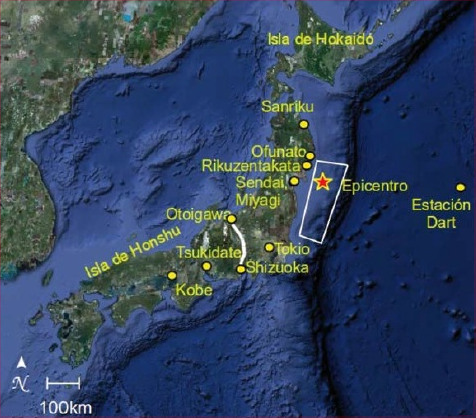
\includegraphics[width=0.4\linewidth]{Epicentro-Sismo.png}
    \caption{Epicentro del sismo}
    \label{Epicentro}
\end{figure}
